\iffalse
\let\negmedspace\undefined
\let\negthickspace\undefined
\documentclass[journal,12pt,twocolumn]{IEEEtran}
\usepackage{cite}
\usepackage{amsmath,amssymb,amsfonts,amsthm}
\usepackage{algorithmic}
\usepackage{graphicx}
\usepackage{textcomp}
\usepackage{xcolor}
\usepackage{txfonts}
\usepackage{listings}
\usepackage{enumitem}
\usepackage{mathtools}
\usepackage{gensymb}
\usepackage{comment}
\usepackage[breaklinks=true]{hyperref}
\usepackage{tkz-euclide} 
\usepackage{listings}
\usepackage{gvv}                                        
\def\inputGnumericTable{}                                 
\usepackage[latin1]{inputenc}                                
\usepackage{color}                                            
\newtheorem{theorem}{Theorem}[section]
\usepackage{array}                                            
\usepackage{longtable}                                       
\usepackage{calc}                                             
\usepackage{multirow}                                         
\usepackage{hhline}                                           
\usepackage{ifthen}                                           
\usepackage{lscape}
\newtheorem{problem}{Problem}
\newtheorem{proposition}{Proposition}[section]
\newtheorem{lemma}{Lemma}[section]
\newtheorem{corollary}[theorem]{Corollary}
\newtheorem{example}{Example}[section]
\newtheorem{definition}[problem]{Definition}
\newcommand{\BEQA}{\begin{eqnarray}}
\newcommand{\EEQA}{\end{eqnarray}}
\newcommand{\define}{\stackrel{\triangle}{=}}
\theoremstyle{remark}
\newtheorem{rem}{Remark}
\begin{document}
\bibliographystyle{IEEEtran}
\vspace{3cm}
\title{GATE 22 EE/46}
\author{EE23BTECH11040 - Manoj Kumar Ambatipudi$^{*}$% <-this % stops a space
}
\maketitle
\newpage
\bigskip
\renewcommand{\thefigure}{\theenumi}
\renewcommand{\thetable}{\theenumi}
\textbf{QUESTION:}
Let a causal LTI system be governed by the following differential equation, 
\begin{align}
    y\brak{t} + \frac{1}{4}\frac{dy}{dt} = 2x\brak{t} \label{eq1}
\end{align}
where $x\brak{t}$ and $y\brak{t}$ are the input and output respectively. It's impulse response is 
\hfill (GATE EE-2022)\\
\fi
\textbf{Solution:}

From \eqref{eq1}, corresponding Laplace transform, 
\begin{align}
    Y\brak{s} + \frac{1}{4}\brak{sY\brak{s} - y\brak{0}} = 2X\brak{s}
\end{align}
Since it is causal LTI system, 
\begin{align}
    y\brak{0} &= 0\\
	\implies Y\brak{s} + \frac{1}{4}sY\brak{s} &= 2X\brak{s}\\
    \implies Y\brak{s} &= X\brak{s}\frac{8}{4 + s}\\
    \implies H\brak{s} &= \frac{8}{4 + s}\quad ROC:Re\brak{s} > -4
\end{align}
Taking inverse laplace transform and applying causality conditions 
\begin{align}
    h\brak{t} = 8e^{-4t}u\brak{t}
\end{align}
\begin{figure}[h]
\renewcommand\thefigure{1}
    \centering
    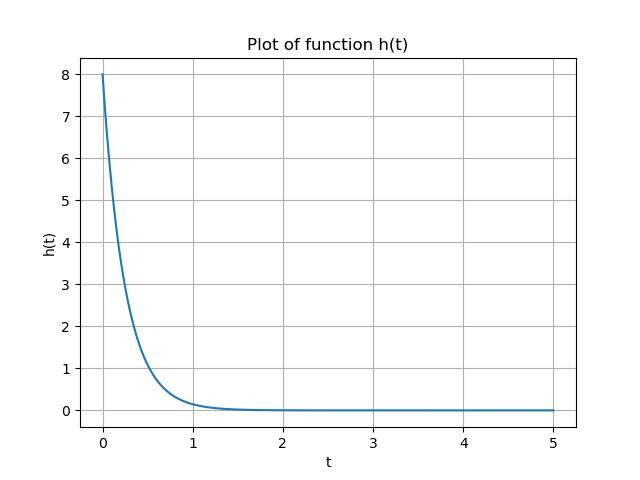
\includegraphics[width=1.0\columnwidth]{2022/EE/46/figs/fig_1.jpg}
    \caption{Plot of $h\brak{n}$, taken from python3}
    \label{fig:1}
\end{figure}
